\documentclass[aspectratio=169, table]{beamer}


%\usepackage[beamertheme=./praditatheme]{Pradita}

\usetheme{Pradita}

\subtitle{IF231303-Software Architecture}
\title{\huge Chapter-9: Mikrokernel\\/Plugin Architecture}
%\date[Serial]{\scriptsize {PRU/SPMI/FR-BM-18/0222}}
\author[Pradita]{\small {\textbf{Paris Matio, Brayan Elmer P, Richard Haryono\\ Alfa Yohannis}}}


\begin{document}
	
	
	\begin{frame}[plain]
		\maketitle
	\end{frame}
	
	% Slide 1: Introduction
	\begin{frame}{Introduction}
		\begin{itemize}
			\item Microkernel/Plugin Architecture is a software design pattern that divides the operating system (OS) into small, modular components.
			\item This presentation discusses the definition, architecture, processes, advantages, disadvantages, and examples of Microkernel/Plugin Architecture in software systems.
		\end{itemize}
	\end{frame}
	
	% Slide 2: Definition
	\begin{frame}{Definition}
		\begin{itemize}
			\item Microkernel/Plugin Architecture is an architectural pattern where the core functionality of the system, known as the microkernel, is kept as minimal as possible.
			\item Additional functionalities are implemented as plugins or modules that can be dynamically loaded and unloaded from the system.
		\end{itemize}
	\end{frame}
	
	% Slide 3: Architecture
	\begin{frame}{Architecture}
		\begin{itemize}
			\item In a Microkernel/Plugin Architecture, the microkernel provides basic services such as memory management, process scheduling, and inter-process communication.
			\item Plugins or modules extend the functionality of the system by providing services such as device drivers, file systems, and network protocols.
		\end{itemize}
	\end{frame}
	
	\begin{frame}{Microkernel in Operation Systems}
		\vspace{20pt}
		\centering		        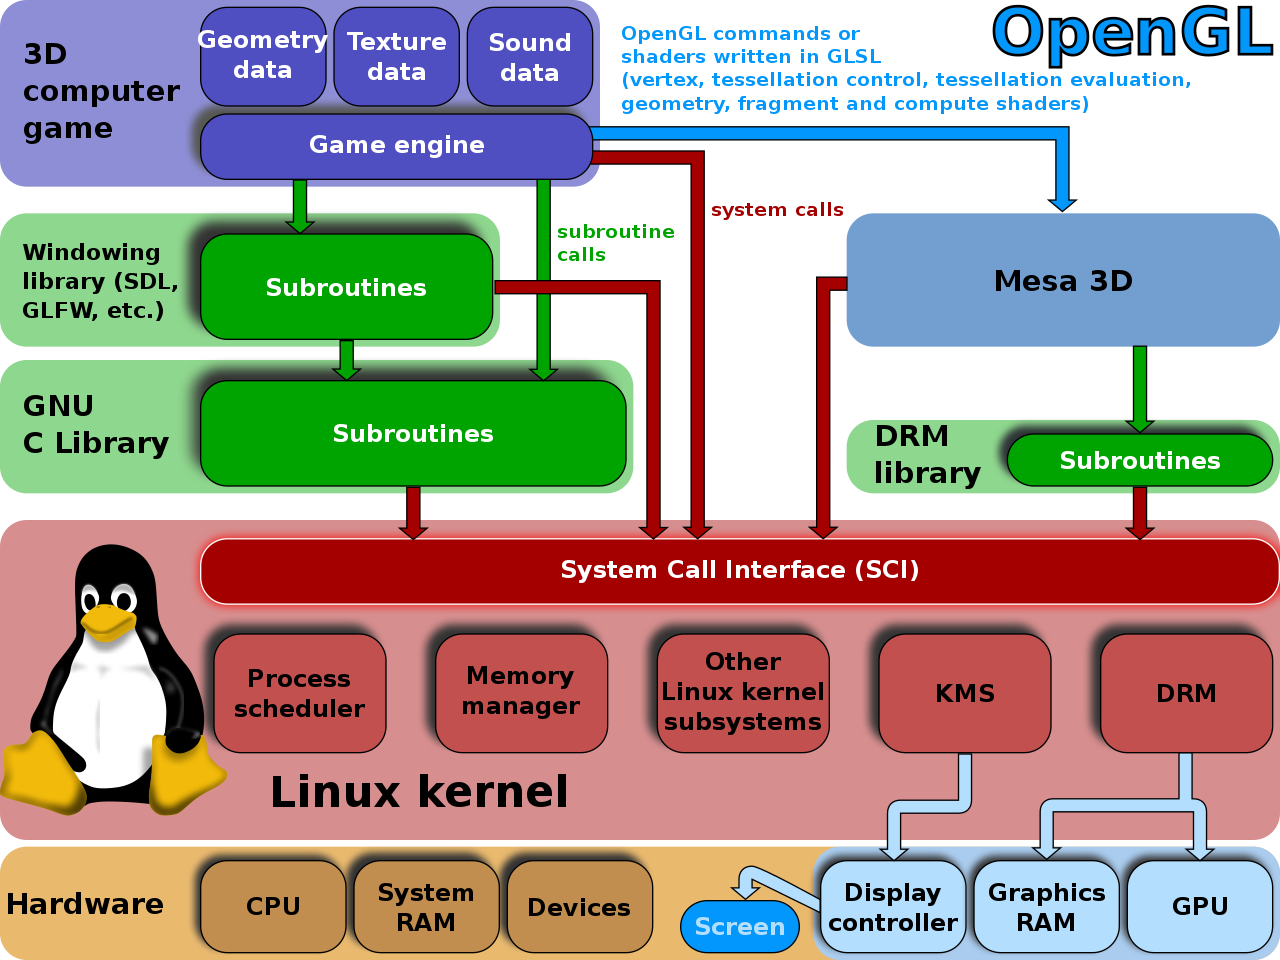
\includegraphics[width=\textwidth]{../../images/microkernel1}
	\end{frame}
	
	
	\begin{frame}{Plugin Architecture}
		\vspace{30pt}
		\centering
		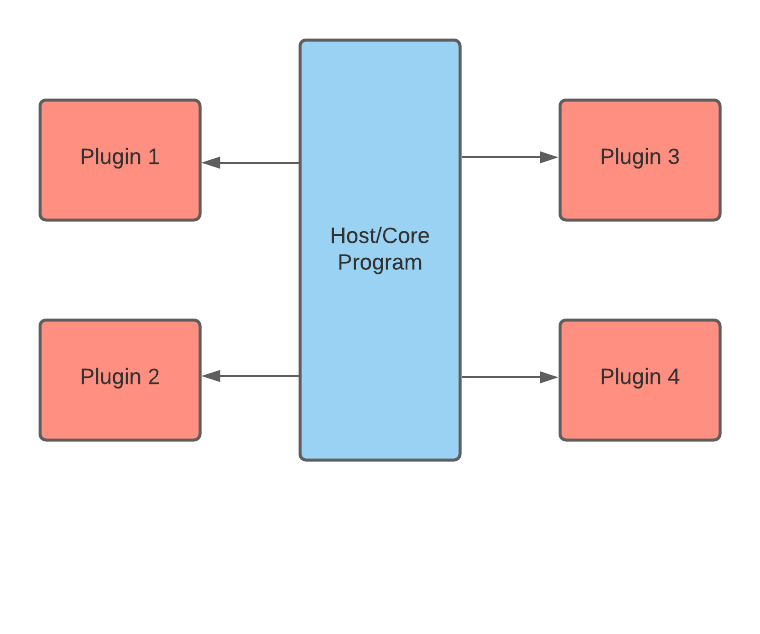
\includegraphics[width=0.7\textwidth]{../../images/plugin2}
	\end{frame}	
	
	
	% Slide 4: Processes
	\begin{frame}{Processes}
		\begin{itemize}
			\item Communication between the microkernel and plugins is typically achieved through message passing or function calls.
			\item Plugins can register themselves with the microkernel and communicate with each other using well-defined interfaces.
		\end{itemize}
	\end{frame}
	
	% Slide 5: Advantages
	\begin{frame}{Advantages}
		\begin{itemize}
			\item Modularity: Microkernel/Plugin Architecture promotes modularity by allowing system components to be developed and maintained independently.
			\item Extensibility: New functionalities can be added to the system without modifying the core microkernel.
			\item Flexibility: The system can be customized by loading and unloading plugins at runtime.
		\end{itemize}
	\end{frame}
	
	% Slide 6: Disadvantages
	\begin{frame}{Disadvantages}
		\begin{itemize}
			\item Performance Overhead: Communication between the microkernel and plugins may introduce performance overhead compared to monolithic architectures.
			\item Complexity: Managing interactions between the microkernel and plugins can be complex, especially in large-scale systems.
			\item Limited Hardware Support: Some hardware functionalities may be difficult to implement as plugins, leading to limited hardware support.
		\end{itemize}
	\end{frame}
	
	% Slide 7: Examples
	\begin{frame}{Examples}
		\begin{itemize}
			\item MINIX: MINIX is a microkernel-based operating system known for its simplicity and modularity. It uses a microkernel architecture with device drivers and file systems implemented as plugins.
			\item Eclipse: Eclipse is an integrated development environment (IDE) that follows a plugin-based architecture. Developers can extend Eclipse's functionality by installing plugins for different programming languages, frameworks, and tools.
		\end{itemize}
	\end{frame}
	
	\begin{frame}{Microkernel in Minix}
		\vspace{20pt}
		\centering
		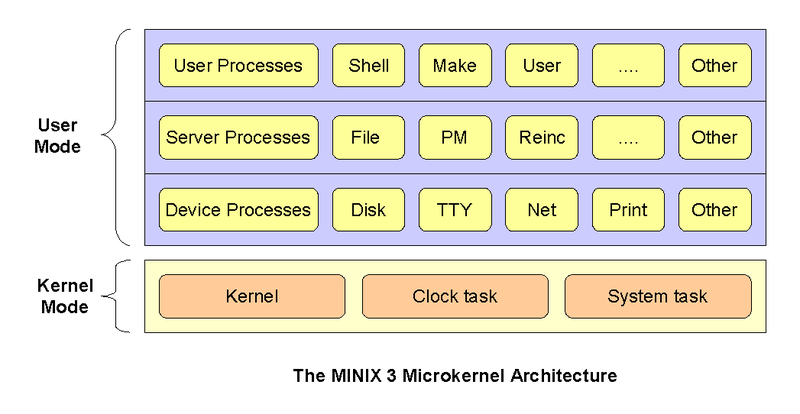
\includegraphics[width=\textwidth]{../../images/microkernel2}
	\end{frame}	
	
	\begin{frame}{Plugin Architecture in Eclipse}
		\vspace{10pt}
		\centering
		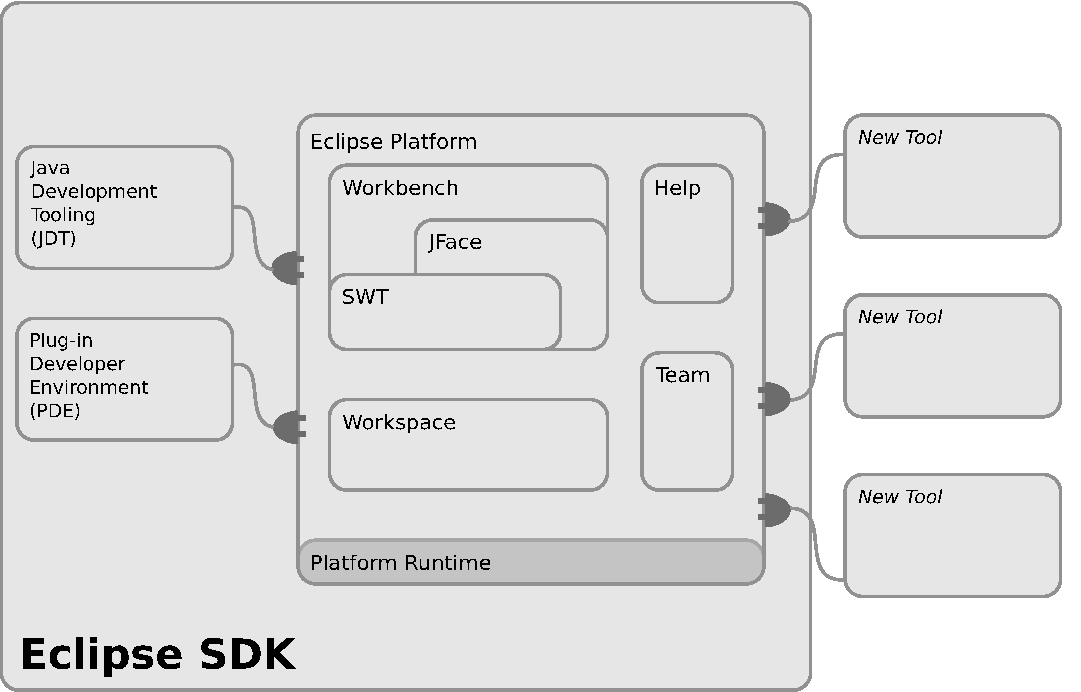
\includegraphics[width=0.78\textwidth]{../../images/plugin1}
	\end{frame}	
	
	% Slide 8: Conclusion
	\begin{frame}{Conclusion}
		\begin{itemize}
			\item Microkernel/Plugin Architecture offers a modular and flexible approach to software design, enabling the development of customizable and extensible systems.
			\item While it has advantages such as modularity and extensibility, it also has drawbacks such as performance overhead and complexity.
			\item Real-world examples such as MINIX and Eclipse demonstrate the practical applications and benefits of Microkernel/Plugin Architecture in software systems.
		\end{itemize}
	\end{frame}
	
\end{document}
